\chapter{Local invariant features}
\section{Derivative of Gaussian filter}
A two-dimensional Gaussian function centered in 0 is obtained as a product of two Gaussians oriented along the $x$ and $y$ axes. Its formula is:
\[G_{\sigma}(x,y) = \frac{1}{2\pi\sigma^{2}}e^{-\frac{x^{2} + y^{2}}{2\sigma^{2}}}\]
\[= \left( \frac{1}{\sqrt{2\pi}\sigma}e^{-\frac{x^{2}}{2\sigma^{2}}}\right) 
    \left( \frac{1}{\sqrt{2\pi}\sigma}e^{-\frac{y^{2}}{2\sigma^{2}}}\right)\]
So you can compute the two-dimensional derivative of Gaussian filter with respect to both $x$ and $y$ directions and combine the output.

\begin{itemize}
    \item $f^{'}_{x}$ (derivative with respect to $x$):
    \[-\frac{x}{2\pi\sigma^4}e^{-\frac{x^2+y^2}{2\sigma^2}}\]
    \item $f^{'}_{y}$ (derivative with respect to $y$):
    \[-\frac{y}{2\pi\sigma^4}e^{-\frac{x^2+y^2}{2\sigma^2}}\]
\end{itemize}
Kernels are an approximation of these derivative functions
\begin{center}
    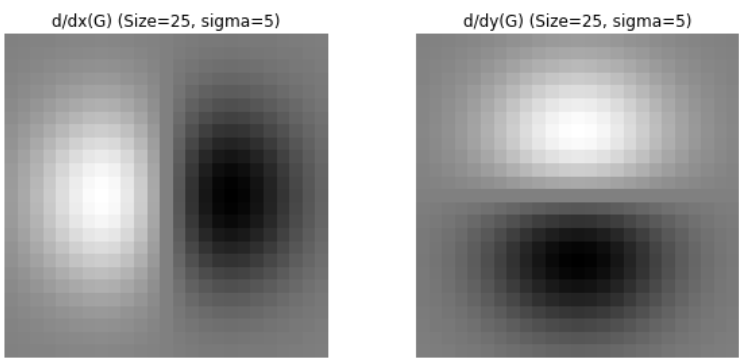
\includegraphics[scale = 0.6]{images/derivative gaussian.png}
\end{center}
Increasing the value of the parameter $\sigma$ means to apply a stronger smoothing effect (remove noise), but it will produce images with more blurred edges. With a low value of $\sigma$ we will be able to detect tiny edges, but with a weaker smoothing effect. This is the reason why $\sigma$ is usually referred as the \textbf{scale of the Gaussian derivative filter}.
\begin{itemize}
    \item Larger values: It detects larger scale edges
    \item Smaller values: It detects finer features
\end{itemize}
We can fine-tune $\sigma$ in order to detect edges at different scales. Basically, fine-tuning the scale could lead to detect edges that are either far \textit{from the camera} (very small) or near (larger).
\section{Examples of 2D derivative filters}
\begin{itemize}
    \item \textbf{Sobel filter:}
    Sobel filter is a derivative filter based on the derivative of Gaussian. It is defined by the following kernels:
    \begin{center}
        \begin{figure}[ht]
        \begin{minipage}{0.45\linewidth}
        \centering
        \begin{tikzpicture}
            \matrix[matrix of nodes ,nodes={minimum size=0.8cm, draw}, row sep=-\pgflinewidth, column sep=-\pgflinewidth](sobel_hz){%
            1 & 0 & -1\\
            2 & 0 & -2\\
            1 & 0 & -1\\
            };
        \end{tikzpicture}
        \caption*{Responds to vertical lines}
        \end{minipage}
        \hspace{20pt}
        \begin{minipage}{0.45\linewidth}
        \centering
        \begin{tikzpicture}
            \matrix[matrix of nodes ,nodes={minimum size=0.8cm, draw}, row sep=-\pgflinewidth, column sep=-\pgflinewidth](sobel_v){%
            1 & 2 & 1\\
            0 & 0 & 0\\
            -1 & -2 & -1\\
            };
        \end{tikzpicture} 
        \caption*{Responds to horizontal lines}
        \end{minipage}
    \end{figure}
    \end{center}
    Let's consider the filter that responds to vertical lines (the same is valid also for the other). It is made of two components.\newline \newline
    The first one is:
    \begin{flushleft}
        \begin{tikzpicture}
        \matrix[matrix of nodes ,nodes={minimum size=0.5cm, draw}, row sep=-\pgflinewidth, column sep=-\pgflinewidth](first_comp){%
        1\\
        2\\
        1\\
        };
        \end{tikzpicture}
    \end{flushleft}
    That is a 1D weighted average filter. \newline\newline 
    The second one is:
    \begin{flushleft}
        \begin{tikzpicture}
        \matrix[matrix of nodes ,nodes={minimum size=0.5cm, draw}, row sep=-\pgflinewidth, column sep=-\pgflinewidth](second_comp){%
        1 & 0 & -1\\
        };
        \end{tikzpicture}
    \end{flushleft}   
    That computes the 1D x-derivative according to the following discrete approximation (1D):
    \[\frac{df}{dx} = f(x+1) - f(x-1) = f^{'}(x)\]
    which is the \textit{central} derivative.\newline
    Thanks to the 1D weighted average component, this filter is less sensitive to noise. In fact, as the Gaussian filter does, it emphasizes pixels near the center of the kernel and has an averaging effect.
    \begin{center}
        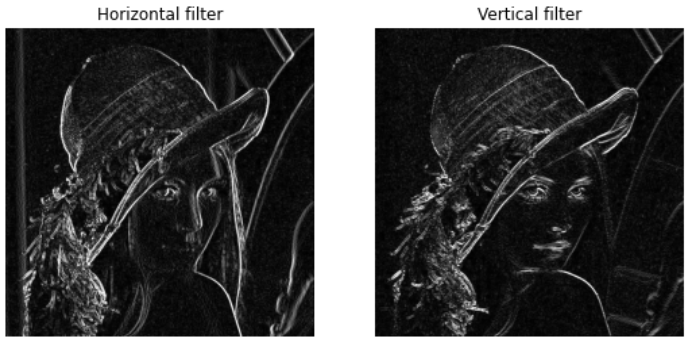
\includegraphics[scale = 0.7]{images/sobel lena.png}
    \end{center}
    \item \textbf{Prewitt filter:}
    Prewitt filter is a derivative filter similar to Sobel but less "sophisticated", because it doesn't have the weighted average component (it does not give more weight to pixels near the center).
    \begin{center}
        \begin{figure}[ht]
        \begin{minipage}{0.45\linewidth}
        \centering
        \begin{tikzpicture}
            \matrix[matrix of nodes ,nodes={minimum size=0.8cm, draw}, row sep=-\pgflinewidth, column sep=-\pgflinewidth](prewitt_hz){%
            1 & 0 & -1\\
            1 & 0 & -1\\
            1 & 0 & -1\\
            };
        \end{tikzpicture}
        \end{minipage}
        \hspace{5pt}
        \begin{minipage}{0.45\linewidth}
        \centering
        \begin{tikzpicture}
            \matrix[matrix of nodes ,nodes={minimum size=0.8cm, draw}, row sep=-\pgflinewidth, column sep=-\pgflinewidth](prewitt_v){%
            1 & 1 & 1\\
            0 & 0 & 0\\
            -1 & -1 & -1\\
            };
        \end{tikzpicture} 
        \end{minipage}
    \end{figure}
    \end{center}
    Let's see an application of this filter:
    \[
    I = 
    \begin{bmatrix}
        10 & 10 & 20 & 20 & 20\\
        10 & 10 & 20 & 20 & 20\\
        10 & 10 & 20 & 20 & 20\\
        10 & 10 & 20 & 20 & 20\\
        10 & 10 & 20 & 20 & 20\\
    \end{bmatrix}
    *\frac{1}{3}
    \begin{bmatrix}
       -1 & 0 & 1\\
       -1 & 0 & 1\\
       -1 & 0 & 1\\
    \end{bmatrix}
    =
    \begin{bmatrix}
       0 & 0 & 0 & 0 & 0\\
       0 & 10 & 10 & 0 & 0\\
       0 & 10 & 10 & 0 & 0\\
       0 & 10 & 10 & 0 & 0\\
       0 & 0 & 0 & 0 & 0\\
    \end{bmatrix}
    \]
    As you can see, it detects a vertical edge in the transition zone between 10 and 20.
    \item \textbf{Scharr filter:}
    Scharr filter is basically a Sobel operator in which central components are more emphasized.
    \begin{center}
        \begin{figure}[ht]
        \begin{minipage}{0.45\linewidth}
        \centering
        \begin{tikzpicture}
            \matrix[matrix of nodes ,nodes={minimum size=0.8cm, draw}, row sep=-\pgflinewidth, column sep=-\pgflinewidth](scharr_hz){%
            3 & 0 & -3\\
            10 & 0 & -10\\
            3 & 0 & -3\\
            };
        \end{tikzpicture}
        \end{minipage}
        \hspace{5pt}
        \begin{minipage}{0.45\linewidth}
        \centering
        \begin{tikzpicture}
            \matrix[matrix of nodes ,nodes={minimum size=0.8cm, draw}, row sep=-\pgflinewidth, column sep=-\pgflinewidth](scharr_v){%
            3 & 10 & 3\\
            0 & 0 & 0\\
            -3 & -10 & -3\\
            };
        \end{tikzpicture} 
        \end{minipage}
    \end{figure}
    \end{center}
    \item \textbf{Roberts filter:} It considers diagonals.
    \begin{center}
        \begin{figure}[ht]
        \begin{minipage}{0.45\linewidth}
        \centering
        \begin{tikzpicture}
            \matrix[matrix of nodes ,nodes={minimum size=0.8cm, draw}, row sep=-\pgflinewidth, column sep=-\pgflinewidth](roberts_hz){%
            0 & 1\\
            -1 & 0\\
            };
        \end{tikzpicture}
        \end{minipage}
        \hspace{5pt}
        \begin{minipage}{0.45\linewidth}
        \centering
        \begin{tikzpicture}
            \matrix[matrix of nodes ,nodes={minimum size=0.8cm, draw}, row sep=-\pgflinewidth, column sep=-\pgflinewidth](roberts_v){%
            1 & 0\\
            0 & -1\\
            };
        \end{tikzpicture} 
        \end{minipage}
    \end{figure}
    \end{center}
\end{itemize}
\section{Canny edge detector}
Canny algorithm is a 4-step edge detection method:
\begin{enumerate}
    \item Application of a Gaussian smoothing filter.
    \item Find magnitude and orientation of gradient by using a first order derivative filter.
    \item Non-maximum suppression: select single maximum, in terms of gradient magnitude, along the orthogonal direction to the edge (non-maximums are set to 0 and only maximums are kept).
    \item Selection of significant edges by \textit{hysteresis} thresholding, which is based (usually) on two thresholds, $T1$ and $T2$, with $T1 > T2$:
    \begin{enumerate}
        \item At the first iteration, only pixels with value $> T1$ are considered "valid"
        \item At the second iteration, pixels with value $< T1$ but $> T2$ are considered valid only if they are adjacent to pixels with value $> T1$.
    \end{enumerate}
\end{enumerate}
\section{Key-points}
Edge detection is useful to extract information, recognize objects, recover geometry and viewpoint, but edges are not very robust against a number of transformations. So, it's not a good idea to use them, for example, for object detection.\newline\newline
Edges are an example of \textbf{key-point}. A key-point is a region of the image in which you have specific properties.
\begin{itemize}
    \item \textbf{flat region:} no change in all direction.
    \item \textbf{edge:} no change along the edge direction.
    \item \textbf{corner:} significant change in all directions.
\end{itemize}
Corners are \textbf{local features} that are more informative and more robust to different image transformations than edges.

\subsection{Why extract key-points from an image ?}
One technique in which is required key-points extraction is \textbf{panorama stitching}, which is basically a method to combine multiple images of the same object. The process can be described in 3 main steps:
\begin{enumerate}
    \item extract key-points: it is necessary an algorithm that is able to detect the same key-points (at the same location) in all the images despite the transformations (different point of view). 
    \item match key-point features.
    \item align images.
\end{enumerate}
\textbf{Other applications:}
\begin{itemize}
    \item Image alignment
    \item 3D reconstruction
    \item Motion tracking
    \item Robot navigation
    \item Indexing and database retrieval
    \item Object recognition
\end{itemize}

\subsection{Characteristics of good key-points}
A good local features should have the following properties:
\begin{itemize}
    \item Repeatability: can be found despite geometric and photometric transformations.
    \item Salience: Each key-point is distinctive.
    \item Compactness and efficiency: many fewer key-points than image pixels.
    \item Locality: key-points are obtained observing a small local area of the original image: therefore more robust to clutter and occlusion.
    
\end{itemize}

\section{Corner detection (Harris corner detector)}
Consider taking an image patch $(x,y) \in W$ (small window) and shifting it by $[u,v]$. The sum of squared differences between the two patches is given by: 
\[E(u,v) = \sum_{(x,y)\in W}[I(x+u, y+v) - I(x,y)]^{2}\]
A corner is a location in which shifting the window in any direction lead to a large change in intensity (high value of $E(u,v)$). We can rewrite $E$ as follows:
\[E(u,v) = \sum_{x,y}W(x,y)[I(x + u, y + v) - I(x,y)]^{2}\]
where $W(x,y)$ is the \textit{window function} that can be:
\begin{itemize}
    \item $W(x,y) = 1$ if $(x,y)$ is a point within the window, 0 otherwise.
    \item Gaussian function that emphasizes more the central pixels of the window.
\end{itemize}
Let's see if the corners extracted by the Harris corner detector are robust against the following geometric transformations:
\begin{itemize}
    \item Translation
    \item Rotation
    \item Scale
\end{itemize}
The algorithm is translation invariant because, despite the specific location of the corner in the image, the information used is centered around the local feature. It is also rotation invariant for the same reason, but it is \textbf{not} scale invariant. This is because if you \textit{zoom-in} or \textit{zoom-out} the original object, what was previously a corner is now probably classified as an edge.

\section{Detect scale invariant features}
\label{section:scale_inv_features}
\textbf{Scale invariant detection goal:} given different images of the same scene with large scale differences between them, find the same key-points independently in each image.\newline\newline
An idea to do it is to generalize the Harris corner detection algorithm such that it is scale invariant. To achieve this goal is necessary a function which is able to automatically adapt the size of an image patch (e.g. a circular region) according to the given scale. Then we can use this scale invariant function to perform automatic scale selection and combine it with the Harris corner detector. 

\subsection{Scale invariant functions}
A good scale invariant function is a function that behaves the same despite the scaling transformation (e.g. reducing by half the size of the original image). Given a local feature at a specific scale, imagine to plot the behavior of a function $f$ on this feature depending on the size of the patch. Then, the "best" patch size for the given scale is the one in which $f$ has the highest response (local max).\newline\newline
So, a good scale invariant function should also have one stable sharp peak.
\subsection{Laplacian of Gaussian (LoG)}
It is possible to design a new filter by computing the second order derivative of Gaussian. This filter is called \textbf{Laplacian of Gaussian} (Mexican hat filter) and is defined as follows:
\[\nabla^{2}G(x,y) = \frac{\partial^{2}G}{\partial x^{2}} + \frac{\partial^{2}G}{\partial y^{2}}\]
\begin{center}
    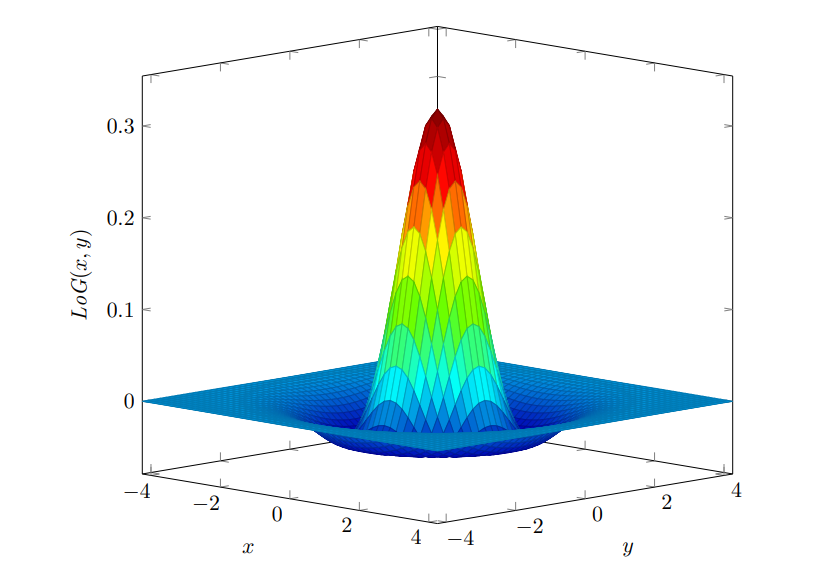
\includegraphics[]{images/LoG.png}
\end{center}
This new operator can be used in order to detect circular regions at different scales (blob detection). Basically, it highlights parts of the image with high contrast around a circular region.
\begin{center}
    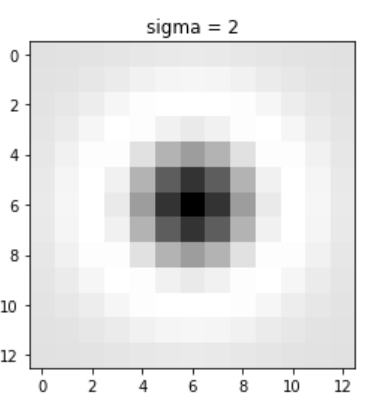
\includegraphics[scale = 0.8]{images/circular region loG.png}
\end{center}
As in the case of the Gaussian filter, we can fine-tune the $\sigma$ parameter in order to make the size of the circular region either bigger or smaller.
\begin{itemize}
    \item Increasing $\sigma$: More blur effect and larger size of the circular region.
    \item Decreasing $\sigma$: Less blur effect and smaller size of the circular region.
\end{itemize}
As usual, the corresponding kernel is a discrete approximation of the continuous function. \newline\newline
So, this filter can be used as the scale invariant function mentioned before, because it gives an high response if the circular region fits well the underlying image region\footnote{giving a high response means that the pixel values in the resulting image after the application of the filter are high.}. In order to find the circular region size that best fits a local feature at a given scale, we can apply this filter for different values of $\sigma$ (ideally all) and look for the one in which the filter gives the highest response.
\begin{center}
    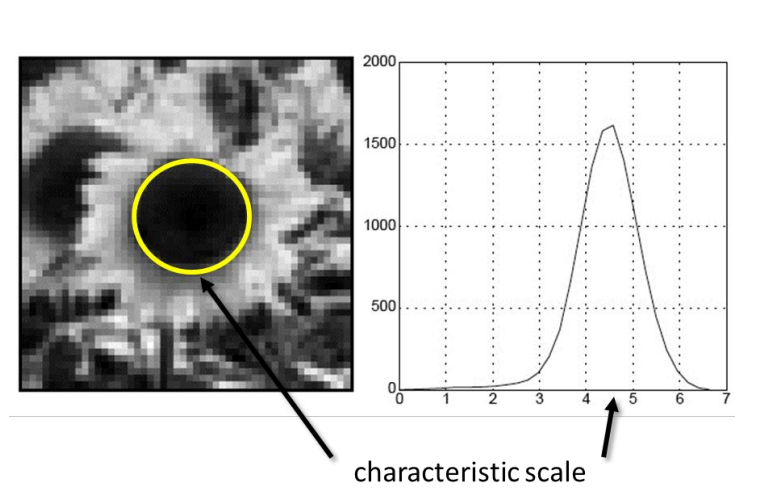
\includegraphics[scale = 0.8]{images/LoG scales.png}
\end{center}
Note that the filter is scale invariant but also rotation invariant, because it considers circular regions.

\subsection{Harris-Laplacian: Scale invariant detection}
Harris-Laplacian is a corner detection algorithm that applies Harris algorithm \textit{in space} (image coordinates) and the Laplacian of Gaussian over the different scales (changing the parameter $\sigma$). It can be used in order to detect local features across scales. \newline\newline
Let's say there is a $3 \times 3$ window. It computes Harris corner detection across different scales (images convolved with $LoG$ filters with different values of $\sigma$) and it detects as a key-point a pixel in which its value is the local maxima in its respective scale \textbf{and} also in the previous scale and in the next one. Basically, a key-point is compared with its respective 8 pixels neighborhood and with the 18 pixels from adjacent scales (9 pixels from each scale).
\begin{center}
    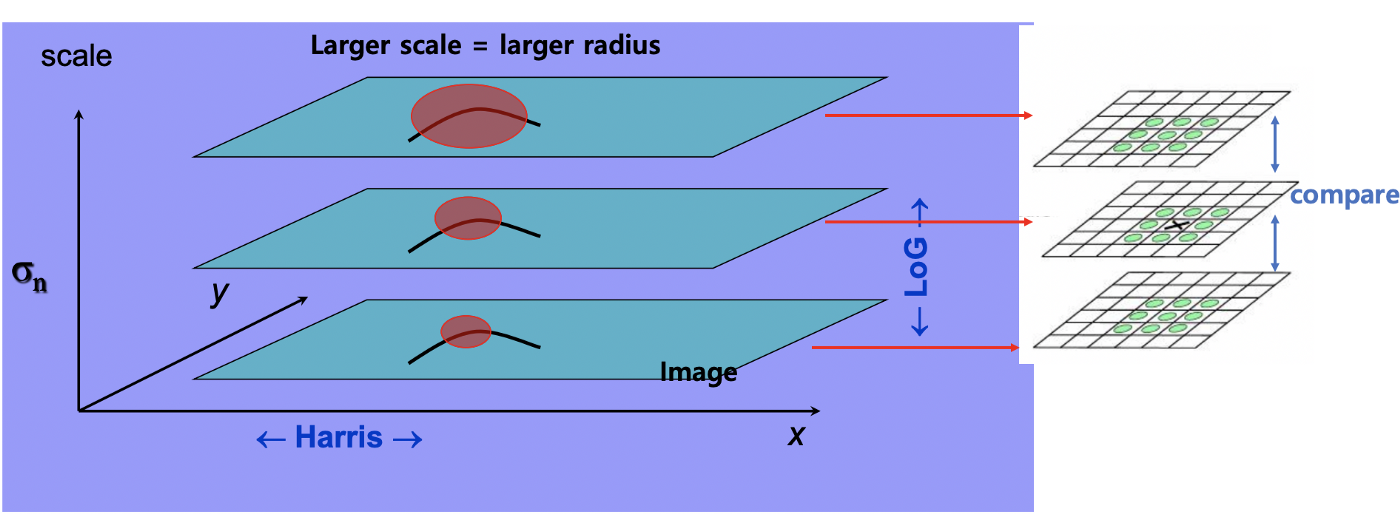
\includegraphics[scale = 0.3]{images/Harris-LoG.png}
\end{center}
This technique makes the Harris detector more robust to the scale changes.

